Context-dependence of gradable adjectives has been promisingly formalized in computational models within the Rational Speech Act framework -  a suite of game-theoretically oriented recursive models of pragmatic language understanding \parencite[e.g.,][]{goodman2016, lassiter2017adjectival, tessler2017warm}. Introduced by \textcite{frank2012predicting}, the Rational Speech Act framework is well in line with recent insights in Bayesian cognitive modelling, showing a great deal of flexibility to account for various phenomena studied in pragmatics like scalar implicature, hyperbolic language or generics, among many others \parencite[e.g.,][]{tenenbaum2011grow, problang}. This chapter reviews the basics of Rational Speech Act models and specifically prior models of gradable adjectives, to finally propose an extension of existing models formalizing the reference-predication trade-off hypothesis.%, allowing to flexibly incorporate reasoning about context and role of the noun in comparison class inference. 
  
\section{Understanding Rational Speech Act Models}

Language is fascinatingly flexible and efficient, and largely so because interlocutors do not have to explicitly encode all information in utterances they produce, but instead rely on each other's ability to infer many aspects of the message from linguistic and situational context. In particular, pragmatic models of communication posit that given these contextual constrains, speakers and listeners can efficiently \emph{reason about each other's intended meaning of utterances} under one important assumption: speakers are approximately \emph{rational} with respect to their communicative goals \parencite{frank2012predicting}. The Rational Speech Act framework (henceforth: RSA) views this process of establishing the intended meaning as recursive reasoning between speaker and listener: in interpretation-oriented models, a pragmatic listener $L_1$ infers a state of the world intended to be conveyed by a rational speaker $S_1$, by using \emph{Bayesian inference} to reason about likely world states given the observed utterance, given that the speaker $S_1$ chooses utterances according to their most likely semantic interpretation by a literal listener $L_0$ \parencite{problang}.  

The idea of language as rational action produced by \emph{cooperative} interlocutors was formulated by \textcite{grice1975logic}. The core of his proposal are four conversational maxims that speakers are thought to stick to when producing utterances in order to convey particular messages: the \emph{maxims of relation} (contributions made to the conversation are relevant), \emph{quantity} (the contributions are as informative as required, but not more so), \emph{quality} (the speaker believes their contributions to be true) and \emph{manner} (the way the contributions are expressed is perspicuous). Listeners then reason about intended messages in light of these maxims \parencite{grice1975logic}.

Grice’s ideas became particularly influential when precise information-theoretic formalisations of such vague concepts like \emph{informativeness, cooperation} and \emph{relevance} were proposed, and, informed by insights from game-theory, gave rise to RSA \parencite{frank2012predicting}.
In particular, RSA captures cooperative coordination of intended meaning between interlocutors via recursive application of probabilistic mechanisms; and relevance or informativeness of utterances is captured as the \emph{utility} of the utterance in helping the listener reduce uncertainty in their beliefs about the world, where these beliefs can be represented as a probability distribution over possible states of the world \parencite[as advocated by e.g.][]{tenenbaum2011grow}.  
That is, listeners update their beliefs about the world via Bayes' rule upon hearing an utterance produced by an informative speaker \parencite{frank2012predicting}.

The mechanisms of RSA are best illustrated by a simple example from a reference game, described by \textcite{frank2012predicting}.
Consider a simple world consisting of a context $C$ = \{blue square, blue circle, green square\} (Fig. \ref{rsa-scene}).
\begin{figure*}[t]
	\begin{center}
		
\includegraphics[width=0.5\linewidth]{rsa_scene.png}
	\end{center}
	\vspace{-0.3cm}
	\caption{A simple reference resolution example scenario: the context $C$ consists of three possible referents \parencite{frank2012predicting}}
	\label{rsa-scene}
\end{figure*}
In a reference game scenario, a speaker wants to communicate to a listener a particular referent $s$ in context $C$, e.g., the blue square. To do so, she has a finite set of utterances $U = \{blue, green, square, circle\}$.\footnote{The finite fixed set of alternative utterances is a crucial assumption made in RSA. It is an important question for future research how interlocutors actually determine this set of relevant alternatives.} A listener then tries to recover the intended referent (i.e., the blue square) upon receiving an utterance (e.g., "blue"). 
As mentioned above, standard RSA models consist of three layers: a pragmatic speaker $S_1$ who chooses an optimal utterance for signalling $s$ (the blue square) to a literal listener $L_0$, who infers all the referents consistent with the literal meaning of the utterance $u$ ('blue'), and a pragmatic listener $L_1$ who reasons about this speaker behaviour given a particular utterance $u$ ('blue'), using Bayes' rule.

So the basis of RSA models is the na\"ive literal listener agent $L_0$ that $S_1$ reasons about when choosing an optimal utterance to communicate the blue square, who computes a probability distribution over possible referents in context $C$  consistent with the received utterance $u$: %\pt{function that maps each utterance to the probability distribution over world states}

$$P_{L_0}(s \mid u, C) = \frac{\llbracket u \rrbracket (s) \times P(s)}{\sum_{s' \in C} \llbracket u \rrbracket (s') P(s')}$$
The context $C$ is typically assumed to be shared between speaker and listener, so it will be dropped in further derivations for simplicity. Given that the denominator is a constant, it can also be dropped for simplicity, so that the probability of a particular state $s$ given utterance $u$ is \emph{proportional} to the literal meaning $\llbracket u \rrbracket (s)$ and the prior probability of $s$: 
$$P_{L_0}(s \mid u) \propto \llbracket u \rrbracket (s) \times P(s)$$
The prior $P(s)$ is the prior belief of $L_0$ about which states are likely to be communicated by the speaker. Typically, a uniform prior is used, indicating that a priori any state is as likely as others, but relevant contextual information like perceptual salience or frequency of some referents might be encoded in this prior \parencite{frank2012predicting}.

The second component of the $L_0$ is the \emph{literal meaning} of the observed utterance $u$ (indicated as $\llbracket u \rrbracket$). In RSA, literal semantics computation is based on a form of Montague’s compositional semantics, typically assuming a mapping from particular states to Boolean truth-values \parencite{montague1973proper} \parencite[but see e.g.][for alternative approaches]{degen2020redundancy}. 
So, for instance for the context Fig. \ref{rsa-scene}, applying the utterance 'circle' to the blue square would return \texttt{false}, but 'blue' would be \texttt{true}:
$$\llbracket circle \rrbracket (blue \: square) = 0$$
$$\llbracket blue \rrbracket (blue\: square) = 1$$
  
So for our example utterance 'blue' the literal listener $L_0$ infers a uniform distribution over the blue circle and the blue square, since the utterance equally applies to both objects (Table \ref{rsa-l0}):

\begin{table}[h]
	\begin{center}
		\caption{The probability distribution over states inferred by $L_0$ when hearing the utterance 'blue' in context $C$.}
		\label{rsa-l0}
		\vskip 0.12in
		\begin{tabular}{cc}
			State & Probability \\
			\hline
			blue circle & 0.5 \\
			blue square & 0.5 \\
			\hline
		\end{tabular}
	\end{center}
\end{table}

The next RSA layer is the pragmatic speaker $S_1$. $S_1$ is modelled as an agent who chooses an utterance $u$ rationally, i.e., according to its expected utility, in order to communicate a particular state of the world $s$ in context $C$ to $L_0$. This is captured in the speaker-utility function $U_{S_1}(u; s)$, which trades-off the informativity of an utterance for $L_0$ with non-negative cost $C(u)$ of producing the particular utterance \parencite{problang}:
$$U_{S_1} (u;s) = log L_0(s \mid u) - C(u)$$
In information-theoretic terms, $L_0$ provides a hook within this utility function to compute the \emph{informativeness} of particular utterances as communicating particular states, 
where informativeness is quantified by surprisal - a measure of how much uttering a particular $u$ reduces uncertainty about the state of the world, given that $u$ is \emph{true of $s$} (i.e., $\llbracket u \rrbracket (s) = 1$) \parencite{frank2012predicting}: 
$$I_{ \tilde{u} (s)}(s) = -log(\tilde{u} (s))$$
$I_{\tilde{u} (s)}(s)$ measures how much information $L_0$ gains when hearing the utterance $u$, assuming a known distribution $\tilde{u} (s)$ over states that are coveyed by the literal interpretation $\llbracket u \rrbracket$ which implies the probability of $s$; i.e., it measures how \emph{surprising} it would be to observe $s$ having observed $u$.
Intuitively, assuming a uniform $\tilde{u} (s)$, the less states an utterance applies to, the lower is the surprisal of a particular state, and the higher is its informativeness. For instance, in the context of Fig.~\ref{rsa-scene}, the utterance 'circle' is highly informative, because there is only one object it applies to, while the utterance 'blue' is less informative because it applies to two objects. 
Therefore, the speaker utility is anti-proportional to the surprisal of the utterance \parencite{frank2012predicting}:
$$U_{S_1} (u;s) = -(-log(\tilde{u}(s))) - C(u) = log L_0(s \mid u) - C(u)$$  %: speakers strive to choose an utterance minimizing surprisal of a particular state of the world given that utterance. 
The cost function $C(u)$ is also an important tool for integrating psychologically plausible information about speaker-biases, like frequency or complexity of producing particular utterances comapred to others. Now the rational speaker $S_1$ maximizes the probability of conveying the intended state of the world $s$ acting according to Bayesian decision theory, by choosing an utterance $u$ proportionally to its expected utility described by the \emph{softmax} function:

$$P_{S_1}(u \mid s) = \frac{e^{\alpha U_{S_1} (u; s)}}{\sum_{u' \in U s.t. u'(s) = true} e^{\alpha U_{S_1} (u'; s)}}$$
The parameter $\alpha$ controls the speaker's \emph{optimality}, assuming $\alpha = 1$ in examples used here; for $\alpha = \infty $ the fully rational decision rule used in game-theory can be recovered \parencite{problang, lassiter2017adjectival}.

For this example, $S_1$ chooses an utterance $u$ maximizing the probability of the state 'blue square' being recovered by $L_0$. So $S_1$ infers a distribution over utterances applicable to the target 'blue square' (Table \ref{rsa-s1}):

\begin{table}[h]
	\begin{center}
		\caption{The probability distribution over utterance inferred by the pragmatic speaker $S_1$ in order to communicate the referent 'blue square'}
		\label{rsa-s1}
		\vskip 0.12in
		\begin{tabular}{cc}
			Utterance & Probability \\
			\hline
			blue & 0.5 \\
			square & 0.5
		\end{tabular}
	\end{center}
\end{table}
 
Finally the top-level layer, the pragmatic listener $L_1$, reasons about this utterance-generating speaker behaviour given a particular utterance $u$ ('blue'), using Bayes' rule:\footnote{This recursive depth of three model layers is a common assumption in RSA models, and requires a reasonable amount of computational resources \parencite{lassiter2017adjectival}. Yet this is just a practical approximation, and some models (e.g., production-oriented models) employ additional levels\parencite{problang}.}
 
$$P_{L_1}(s \mid u) = \frac{P_{S_1}(u \mid s) P(s)}{\sum_{s' \in C} P_{S_1}(u \mid s') P(s')}$$
That is, the probability of a particular state $s$ (i.e., blue square) given the utterance $u$ ('blue') is equal to the probability that the pragmatic speaker $S_1$ would choose $blue$ in order to convey the \textit{blue square}, multiplied by the prior probability $P(s)$ of occurence of state $s = blue \:square$, normalised by a constant sum of probabilities of all possible speaker behaviors for all possible states $s'$. Since the denominator is a constant, it can be dropped, resulting in the probability of a particular $s$ given $u$ being \emph{proportional} to the speaker production probability $P_{S_1}(u \mid s)$ times the state prior $P(s)$:
$$P_{L_1}(s \mid u) \propto P_{S_1}(u \mid s) P(s)$$ 
Interestingly, the state prior $P(s)$ might differ between $L_0$ and $L_1$, e.g. incorporating prior world knowledge of the pragmatic agent $L_1$, but being uniform for the na\"ive agent $L_0$ \parencite{problang}. 

In this example, upon hearing 'blue', $L_1$ infers that the speaker is more likely to convey the blue square (Table \ref{rsa-l1}):

\begin{table}[h]
	\begin{center}
		\caption{The probability distribution over referents inferred by the pragmatic listener $L_1$ upon hearing the utterance 'blue'.}
		\label{rsa-l1}
		\vskip 0.12in
		\begin{tabular}{cc}
			State & Probability \\
			\hline
			blue square & 0.6 \\
			blue circle & 0.4
		\end{tabular}
	\end{center}
\end{table}
\begin{figure*}[t]
	\begin{center}
		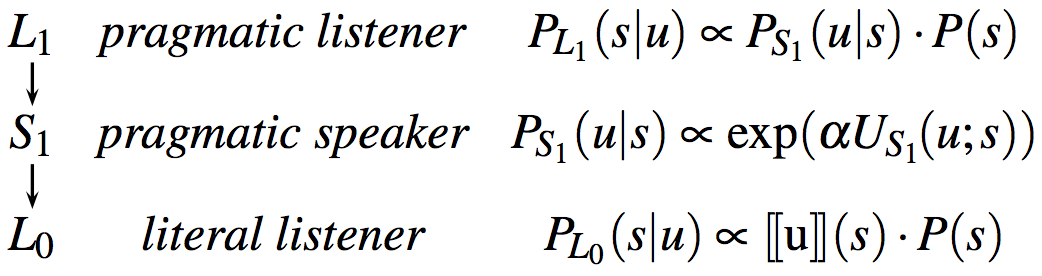
\includegraphics[width=0.5\linewidth]{vanilla-rsa.png}
	\end{center}
	\vspace{-0.3cm}
	\caption{A schematic depiction of a vanilla RSA model \parencite{problang}}
	\label{vanilla-rsa}
\end{figure*}
Putting all the elements together results in the vanilla version of an RSA-model (Fig.~\ref{vanilla-rsa}).
The crucial illustration of the RSA mechanism is the difference between the distributions inferred by $L_0$ and $L_1$ upon observing the same utterance 'blue'. Reasoning about the utterance-generating speaker-model incorporated in $L_1$, while $L_0$ acts according to literal semantics only, is crucial for the pattern of interpretation we observe: $L_1$ infers that the speaker is more likely to mean the blue square, because if she had meant the blue circle, she could have said 'circle', which would have been less ambiguous, and therefore more informative (Table \ref{rsa-l1}). That is, $L_1$ does not only consider what the speaker actually said, but also what the speaker \emph{could have said}. In contrast, $L_0$ infers equal probabilities of 'blue' meaning 'blue square' or 'blue circle' because the utterance is literally true of both referents (Table \ref{rsa-l0}). Crucially, this pattern predicted by the RSA-model is well in line with rational behaviour of humans gathered empirically in such reference game scenarios, showing that human interlocutors make use of more than just the literal semantics of their words when communicating \parencite{frank2012predicting, problang}.

%Having set the basic building blocks of RSA models, some more sophisticated features of RSA relevant for modelling adjectives should be mentioned. 

%note that these exist as part of L1's reasoning \parencite{lassiter2017adjectival}
\section{Previous RSA models of gradable adjectives}
In this section, previous RSA models of gradable adjectives are discussed, which showed that RSA is a flexible tool suitable to integrate more complex pragmatic reasoning required for interpreting vague expressions.
%threshold semantics, where the threshold is probabilistically inferred \parencite{lassiter2017adjectival} for a given comparison class.

\textcite{lassiter2013context} first provided a model of gradable adjective interpretation within the RSA-framework, showing that pragmatic reasoning can capture their meaning via inference over the latent standard of comparison variable $\theta$ underlying the vague semantics (s. Chapter \ref{chapter02}). %Importantly, probabilistic reasoning provides tools to capture uncertainty over certain aspects of the message, in this particular case - the speaker’s intended meaning of the adjectival utterance.  
The proposed model builds upon the standard RSA model with three levels, adding one crucial extension: the pragmatic listener $L_1$ jointly infers the value of the threshold $\theta$ along with the state of the world $s$ (i.e., the degree to which a referent possesses the property described by the adjective):

$$P_{L_1} (s, \theta \mid u) \propto P_{S_1} (u \mid s, \theta) \times P (s) \times P(\theta)$$ 

The model formalized literal meaning of gradable adjectives in terms of degree-semantics, assuming that the lexical entry of the adjective specifies the underlying scale and its polarity (cf. Chapter~\ref{chapter02}):
$$\llbracket u \rrbracket_{\theta} (s) = s > \theta$$
However, the literal meaning of the adjective by itself is underspecified - it depends on the pragmatically recovered threshold $\theta$, which in turn depends on the comparison class used in the particular context; yet, like vanilla RSA the model is anchored in the literal interpretation of the adjective applied to a referent at the level of $L_0$.  
So in order to allow specifying the $L_0$ which requires computating the truth-value of an utterance for a given state, the authors proposed $L_1$ consider all possible assignments of the latent variable value $\theta$, given a prior over that variable $P(\theta)$. Crucially, the state prior $P(s)$ encoded prior knowledge about \emph{likely property degrees for a specific comparison class} which the referent might have. For instance, the difference in the meanings of \emph{big} in 'big for a tree' and 'big for a pug' would be encoded in different priors over the likely properties of the respective referents. It is common practice to quantify this prior knowledge empirically via prior elicitation experiments \parencite{problang}. A uniform $P(\theta)$ encoded that a priori any property degree might qualify for being described by the adjective. 

The assumed $\theta$ values are then iteratively passed down through the model. Given a particular value, the speaker-model can be specified:
$$P_{S_1} (u \mid s, \theta) \propto exp(\alpha \: log (P_{L_0} (s \mid u, \theta) - C(u)) )$$

Then, in contrast to $L_1$ who is uncertain about $\theta$, $L_0$ interprets the utterance literally, so she gets $\theta$ passed down and infers the state distribution consistent with this particular $\theta$ assignment and the observed adjective $u$:
$$P_{L_0} (s \mid u, \theta) = P_{L_0} (s \mid \llbracket u \rrbracket ^\theta = 1 ) \propto \llbracket u \rrbracket ^\theta (s) \times P(s)$$

So putting all the layers together, $L_1$ can compute a joint posterior distribution over all possible combinations of states and values of the latent threshold $\theta$ lifted to the level of the pragmatic listener. Notably, \textcite{lassiter2013context} assumed the relevant comparison class to be supplied to the listener, such that she was uncertain only about the standard of comparison. Yet as discussed in Chapter \ref{chapter03} and shown empirically in Chapter \ref{chapter04}, listeners flexibly reason about the intended comparison class because there might be multiple a priori plausible options in absence of an explicit \emph{for}-phrase.

\textcite{tessler2017warm} introduced an RSA-model of gradable adjectives accounting for flexible reasoning about the relevant comparison class via world knowledge (the rationale and behavioural experiments of this study are described in detail in Section~\ref{2.4.}). In particular, in the proposed model the listener is not only uncertain about the standard of comparison $\theta$, but also about the specificity of the relevant comparison class $c$ (superordinate~vs.~subordinate category of the referent), given prior knowledge about typical property distributions in each category. That is, listeners were assumed to know the a priori probability that an adjective could felicitously apply to a referent given its category, assuming a specific comparison class; they used this knowledge to infer the intended comparison class upon hearing a simple adjectival utterance $u$ of the form '\emph{PRON} is \emph{ADJ}' said of a referent whose \emph{subordinate category was known to the listener}.
Similarly to the model proposed by \textcite{lassiter2013context}, the pragmatic listener iterated over all possible value assignments of the lifted $\theta$ variable when reasoning about the utterance-generating process, to jointly infer the property degree $s$, the threshold $\theta$ and the relevant comparison class $c$, given the utterance $u$:

$$P_{L_1}(s, \theta, c \mid u) \propto P_{S_1} ( u \mid s, \theta, c) \times P(s \mid c_{sub}) \times P(c) \times P(\theta)$$  
That is, the listener reasoned about how a rational speaker $P_{S_1}$ would behave in order to communicate a specific property, given a comparison class and a threshold, together with their prior knowledge about what property degrees are plausible given the subordinate category $P(s \mid c _{sub})$ the referent belongs to, and their prior beliefs $P(c)$ about which comparison class categories are likely to be used and what properties are likely to qualify for applying the adjective ($P(\theta)$). Accordingly, the speaker-model $P_{S_1}( u \mid s, \theta, c)$ can be specified assuming particular values of the property, the comparison class and the threshold:

$$P_{S_1}( u \mid s, \theta, c) \propto exp(\alpha \: log P_{L_0} (s \mid u, \theta, c))$$

The $L_0$ again specifies a literal listener who interprets the adjective $u$ according to its literal semantics, assuming a particular comparison class $c$ and $\theta$:

$$P_{L_0}(s \mid u, \theta, c) \propto \llbracket u \rrbracket_{\theta} (s) \times P( s \mid c)$$  
Importantly, $L_0$ now samples states according to a prior $P(s|c)$ specified by the received comparison class $c$, which integrates the comparison class into the literal semantics. 

Since the predictions of this model strongly depend on prior world knowledge, it is important how the property priors given different comparison classes are specified. \textcite{tessler2017warm} fixed superordinate property distributions as $\mathcal{N} (0, 1)$ and subordinate property distributions as $\mathcal{N}(\mu_{sub}, \sigma_{sub})$, inferring the paramters of subordinate distributions from experimental data. The comparison class prior $P(c)$ was approxiamted as empirical Google WebGram frequencies of usage of the respective comparison class labels. 

\textcite{tessler2017warm} showed that the model captures human inferences discussed in Chapter \ref{2.4.} very well, confirming the role of world knowledge for comparison class inference. 
% potential spot to integrate Dan Yurovsky's work 
However, this model only considered the effect of world knowledge on comparison class inference, and focused on interpretation of simple underspecified utterances of the form 'He is tall'. In the following section, a further extension of previous RSA models is proposed, which accounts for more complex sentences containing a noun and integrates more sophisticated reasoning about several effects contributing to comparison class inference.  

\section{Refpred-RSA}
This section outlines a novel model formalizing the reference-predication trade-off hypothesis.

First, let's recall the reference-predication trade-off hypothesis: it posits that speakers pursue particular \emph{informational goals --- reference} and \emph{predication} --- when crafting their utterances. These informational goals are realized syntactically via different positions of the noun: the noun is more likely to contribute to reference when appearing in the sentence subject, but less likely to do so when appearing in the predicate, hence being more likely to contribute to predication --- i.e., constrain the comparison class. Listeners, in turn, reason about these speaker goals %and expect these particular syntactic realizations 
when interpreting the observed utterance.  
Therefore, the degree to which the noun of the sentence constrains the comparison class --- i.e., serves predication --- trades off with its utility in reference. 

Reasoning about particular informational, or conversational, goals is closely related to basic assumptions made in RSA.
As pointed out above, the speaker is assumed to be a rational agent producing utterances of optimal utility with respect to some specific \emph{conversational goal} determined by discourse, also called \emph{question under discussion (QUD)}  \parencite{lassiter2017adjectival, roberts2012information}. The communication is structured so as to maximize the probability that the listener infers the intended \emph{answer to this QUD}. In the vanilla example used above, the QUD was to determine the intended referent, and the intended answer was 'blue square'. From this perspective, interlocutors' contributions to discourse are \emph{relevant} if and only if they contribute to answering the question under discussion \parencite{roberts2012information}. Note that such questions under discussions might indeed be realized by specific speech acts, but do not have to be - they often remain implicit, and resemble questions rather formally in that they proffer the set of relevant alternatives interlocutors commit to addressing. Yet, interlocutors are fascinatingly good at determining the QUD pragmatically so as to functionally organize their communication around the QUD; they might do so using different strategies, one prominent strategy in English being to make use of focus \parencite{roberts2012information, krifka2008basic}. But they might also employ other strategies, like choosing particular syntactic structures over others, e.g., as proposed by the reference-predication trade-off hypothesis.  

From a semantic perspective, utterances then might have several dimensions of interpretation, each dimension corresponding to the interpretation of the utterance as satisfying a distinct communicative goal, or answering a distinct QUD. This idea was first formlazed within the RSA-framework by \textcite{kao2014nonliteral}, applied to hyperbolic and pragmatic halo effects in interpretation of number words. The crucial novelty they introduced was listener uncertainty about the relevant QUD, deploying multi-dimensional literal meaning of utterances satisfying distinct potential QUDs \parencite{kao2014nonliteral}. 

Yet the majority of RSA models usually assumed that speakers address one particular conversational goal. The listener might be uncertain about it, as in case of QUD-models, or the model might just addressed one pre-defined aspect of communication, i.e., one QUD \parencite[see][for an excellent overview]{problang}. However, this work has shown that interlocutors at least consider multiple informational goals that might be addressed within the same utterance, where different parts of the utterance might probabilistically contribute to achieving each of the goals. Therefore, the model proposed in the following describes speakers' choice of utterances as incremental, where the subject is chosen so as to establich reference, and the predicate is chosen to convey the comparison class --- and so one utterance fulfills multiple QUDs. 
